\chapter{Deep Learning \ac{PSD}}
The primary objective of this analysis is the exploration and implementation of a deep learning architecture for \ac{PSD}. The logical framework of this research follows a sequential paradigm centered on latent feature extraction. Initially, the model is trained in an unsupervised regime to faithfully reconstruct the temporal evolution of the input waveforms. Achieving a low reconstruction error ensures that the latent space, generated by the encoder network, efficiently compresses the information, yielding a highly representative embedding of the underlying signal topologies. 

Exploiting the properties of this manifold, the investigation subsequently shifts to a classification task, aiming to robustly discriminate \ac{SSE} from \ac{MSE}. The fundamental hypothesis is that a non-linear, multivariate mapping of the entire waveform can match or exceed the discrimination efficiency of standard techniques, such as the empirical \ac{AE} analysis. 

Ultimately, this work seeks to decode the latent space itself, exploring potential correlations between the extracted features and specific physical variables of the interaction. This approach is intended to provide a novel interpretive tool for modeling charge collection dynamics within the detector.

Although standard Autoencoders (AEs) provide a robust framework for dimensionality reduction, they inherently map high-dimensional inputs to deterministic, discrete points within the latent space. This deterministic formulation frequently yields a highly fragmented and entangled latent topology, severely limiting the network ability to correlate learned features with underlying physical parameters. Conversely, the Variational Autoencoder (VAE) addresses these limitations by encoding inputs into probabilistic distributions rather than isolated vectors. Specifically, the encoder network does not output a single deterministic coordinate, but rather two distinct statistical parameters: a mean ($\mu$) and a variance ($\sigma^2$ or log($\sigma^2$)). The actual latent representation $z$ is then dynamically sampled from this multi-dimensional Gaussian distribution using the reparameterization trick. 

To prevent these learned distributions from collapsing or behaving arbitrarily, the VAE objective function is regularized by the Kullback-Leibler (KL) divergence. The KL divergence is a statistical metric that quantifies the difference between the network encoded posterior distribution and a chosen prior reference distribution, typically a standard multivariate Gaussian $\mathcal{N}(0, I)$. By heavily penalizing deviations from this prior, the KL term acts as a powerful regularizer, forcing the latent space to be continuous, smooth, and well-structured, thereby ensuring that physically similar waveforms are mapped in close proximity.

In the context of semiconductor signal processing and waveform analysis, this probabilistic approach is critically enhanced by adopting a $\beta$-VAE architecture. A $\beta$-VAE introduces an adjustable hyperparameter, $\beta > 1$, which artificially amplifies the weight of the KL divergence term in the loss function. This intensified regularization places a tighter constraint on the latent channel capacity, forcing the network to learn only the most statistically independent and fundamental generative factors of the data. For Germanium detector signals, this property is vital: it actively promotes disentanglement, preventing the network from confounding distinct physical phenomena -such as total energy deposition, rise time kinetics, and electronic noise- into a single tangled variable. Consequently, the $\beta$-VAE enables a rigorous, interpretable mapping where individual latent nodes correspond to isolated physical observables, thereby providing a significantly more reliable foundation for downstream classification tasks such as \ac{PSD}.
\section{Data cleaning}
\label{sec:data-cleaning}
The data used for this work come from the \textbf{\textit{prl25 version}}, the one used for the LEGEND-200 article \cite{L200-sep25}, period p0?, runs from r000 to r??? and specifically only ICPC data have been used
\begin{figure}[H]
    \centering
    
    % --- Prima figura (a) ---
    \begin{subfigure}[H]{0.45\textwidth}
        \centering
        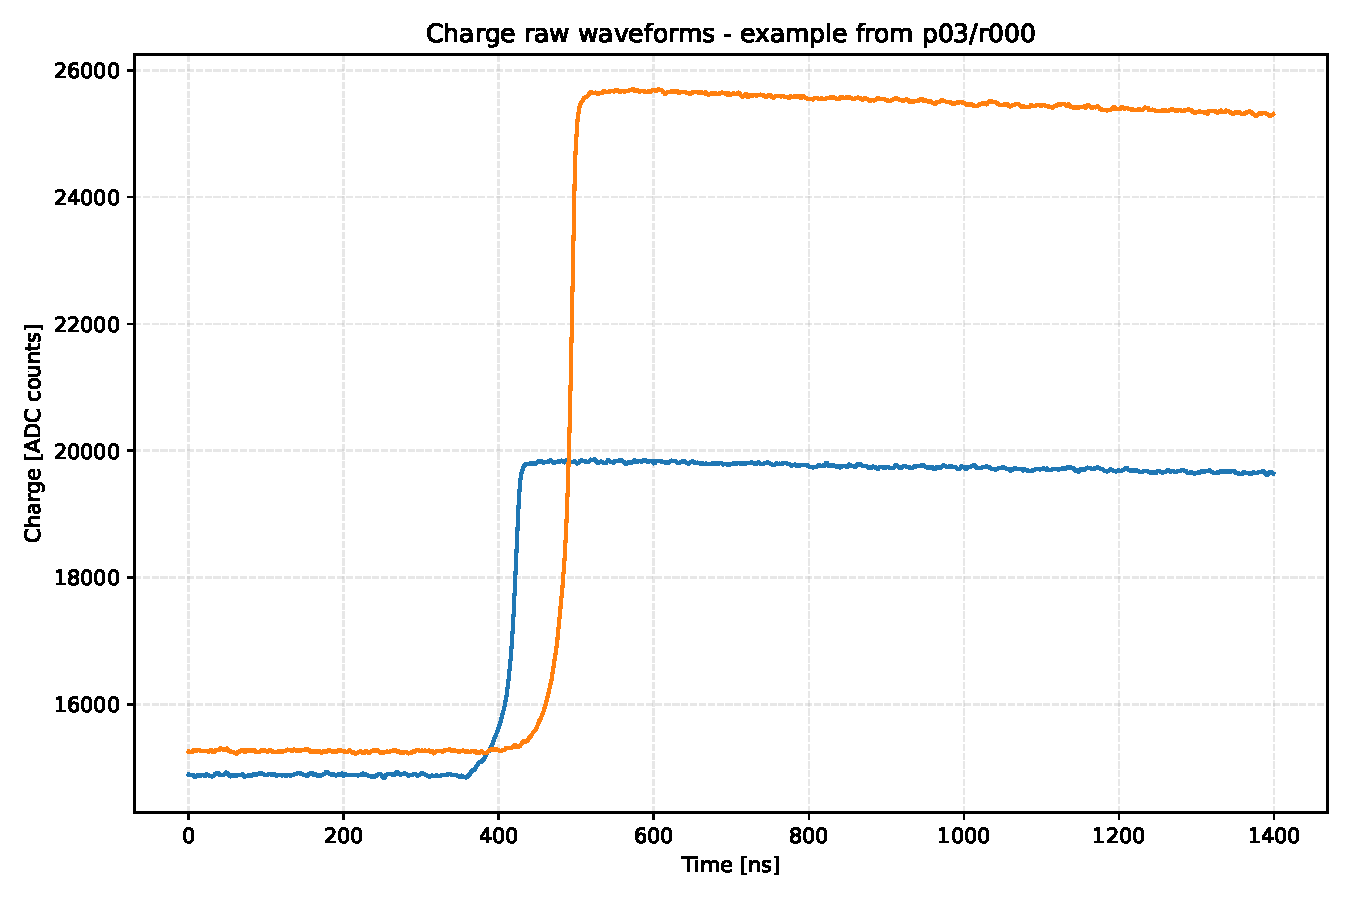
\includegraphics[width=\textwidth]{plots/raw_wf.pdf}
        \caption{Raw charge waveforms.}
        \label{fig:a-raw-wf}
    \end{subfigure}
    \hfill % Crea uno spazio orizzontale tra le due figure affiancate
    % --- Seconda figura (b) ---
    \begin{subfigure}[H]{0.45\textwidth}
        \centering
        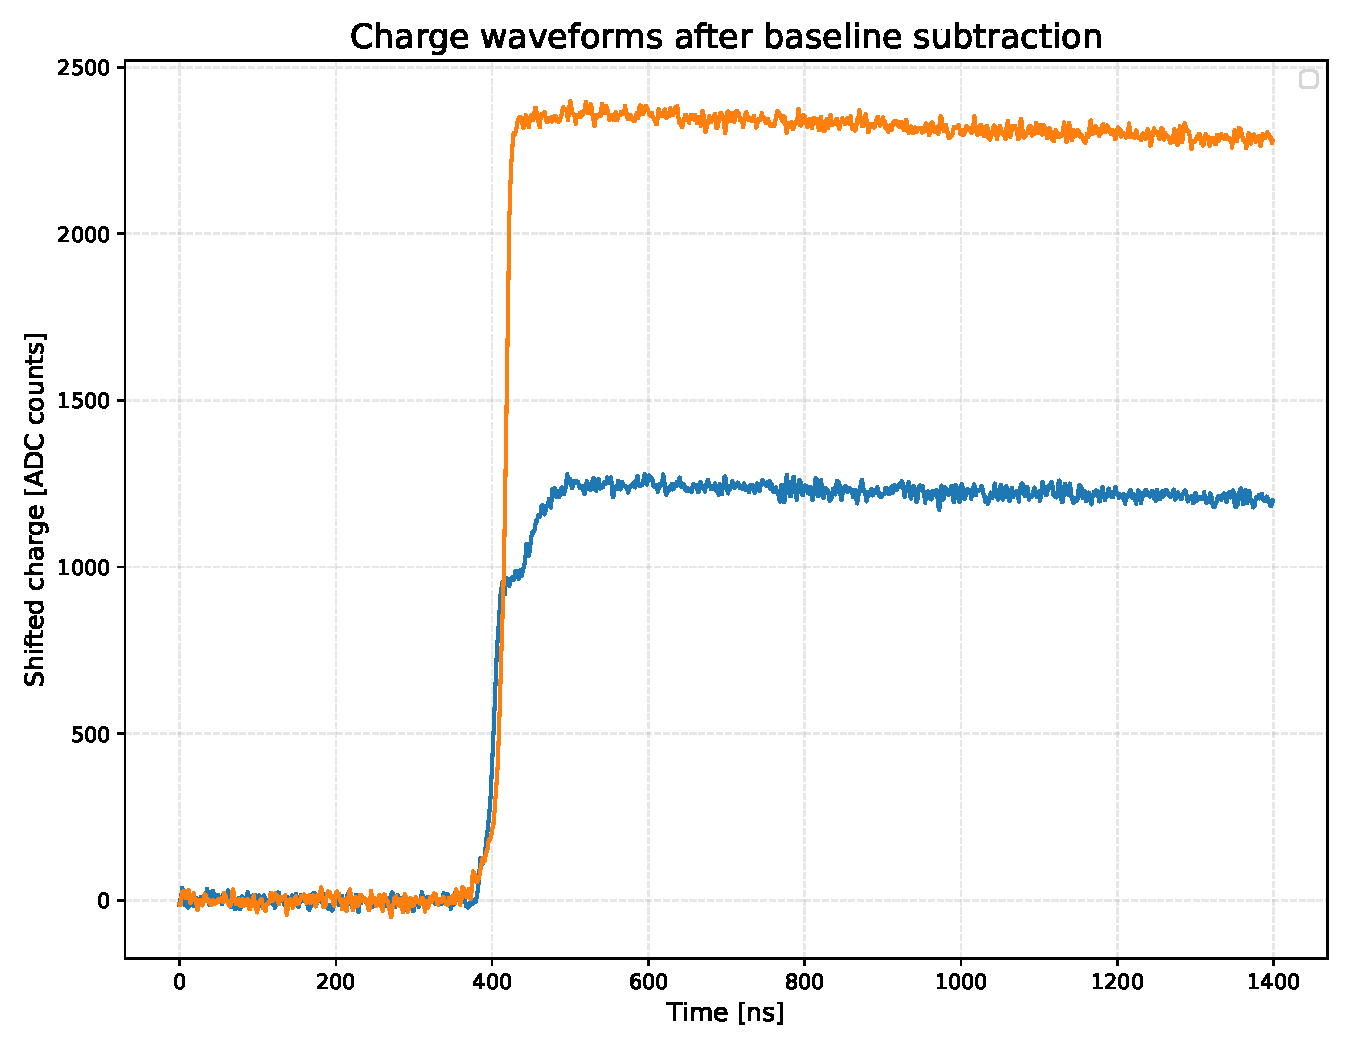
\includegraphics[width=\textwidth]{plots/baseline_subtracted_wf.pdf}
        \caption{Charge waveforms after baseline subtraction.}
        \label{fig:b-baseline}
    \end{subfigure}
    
    \vspace{0.5cm} % Spazio verticale tra la prima e la seconda riga
    
    % --- Terza figura (c) ---
    \begin{subfigure}[H]{0.45\textwidth}
        \centering
        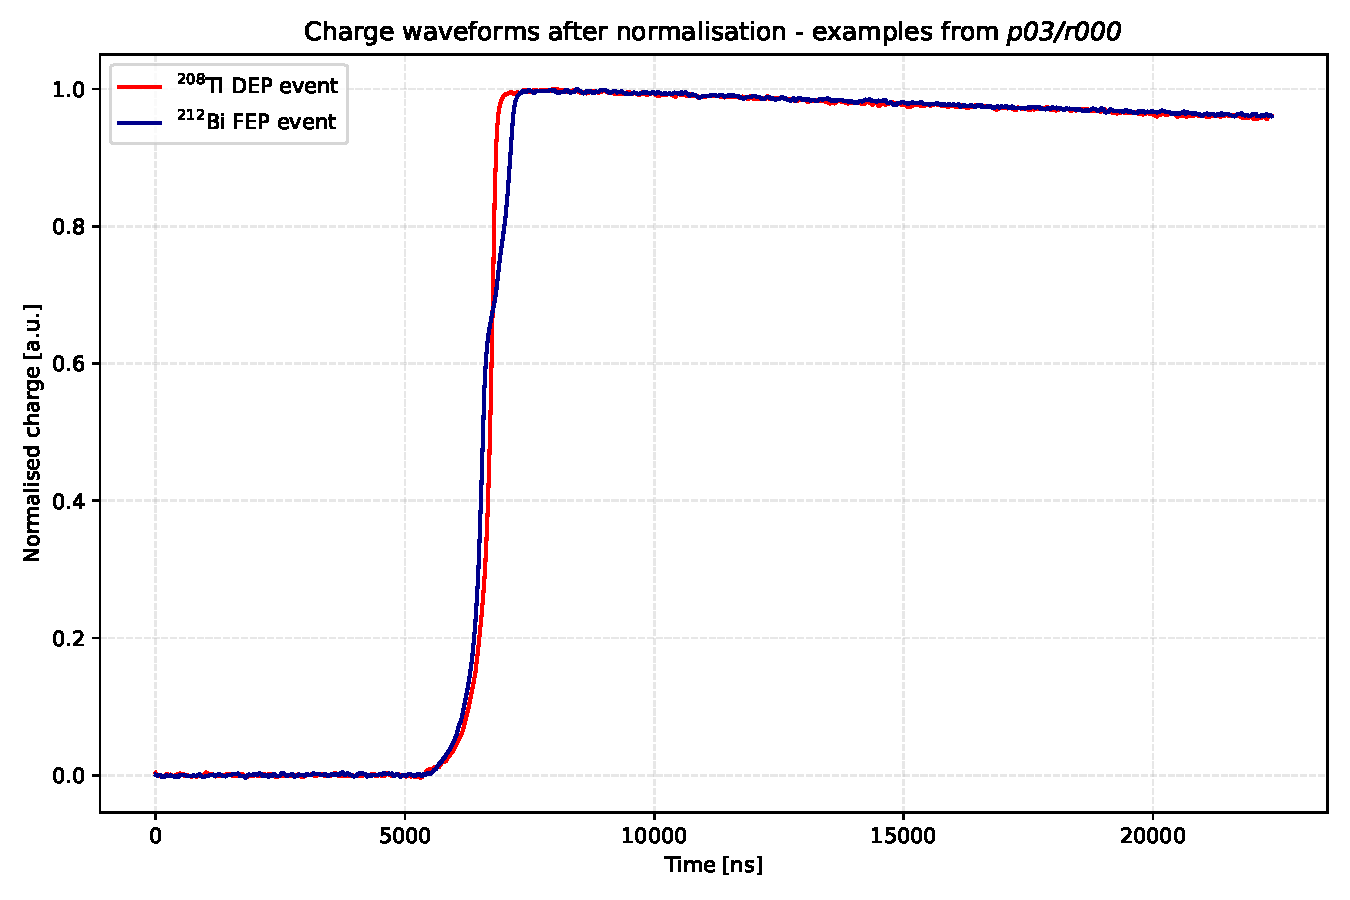
\includegraphics[width=\textwidth]{plots/normalised_wf.pdf}
        \caption{Charge waveforms after normalisation.}
        \label{fig:c-normalised}
    \end{subfigure}
    \hfill
    % --- Quarta figura (d) ---
    \begin{subfigure}[H]{0.45\textwidth}
        \centering
        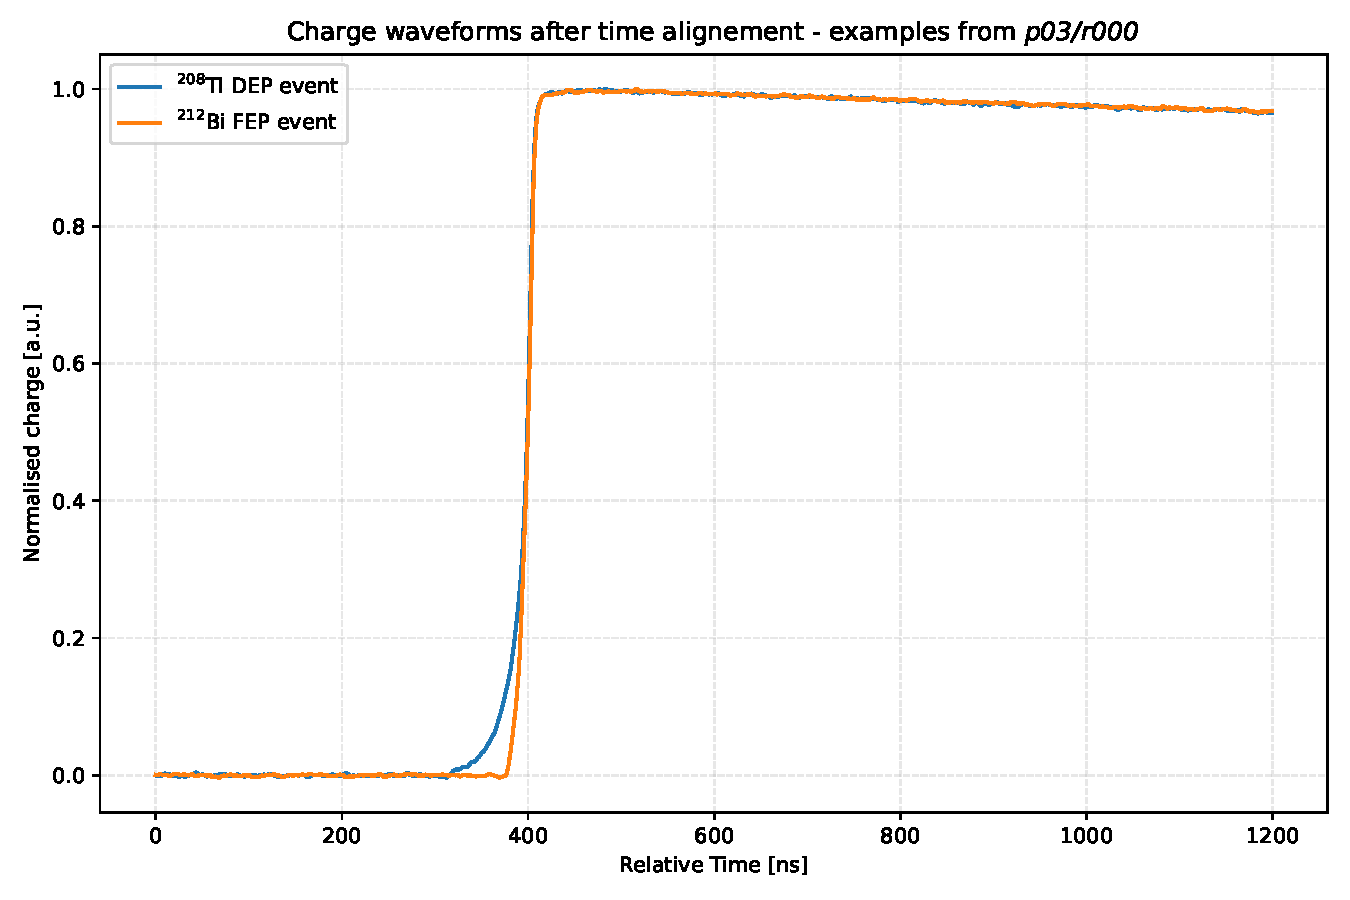
\includegraphics[width=\textwidth]{plots/aligned_wf.pdf}
        \caption{Charge waveforms after time alignement.}
        \label{fig:d-aligned}
    \end{subfigure}

        % --- Quinta figura (e) ---
    \begin{subfigure}[H]{0.45\textwidth}
        \centering
        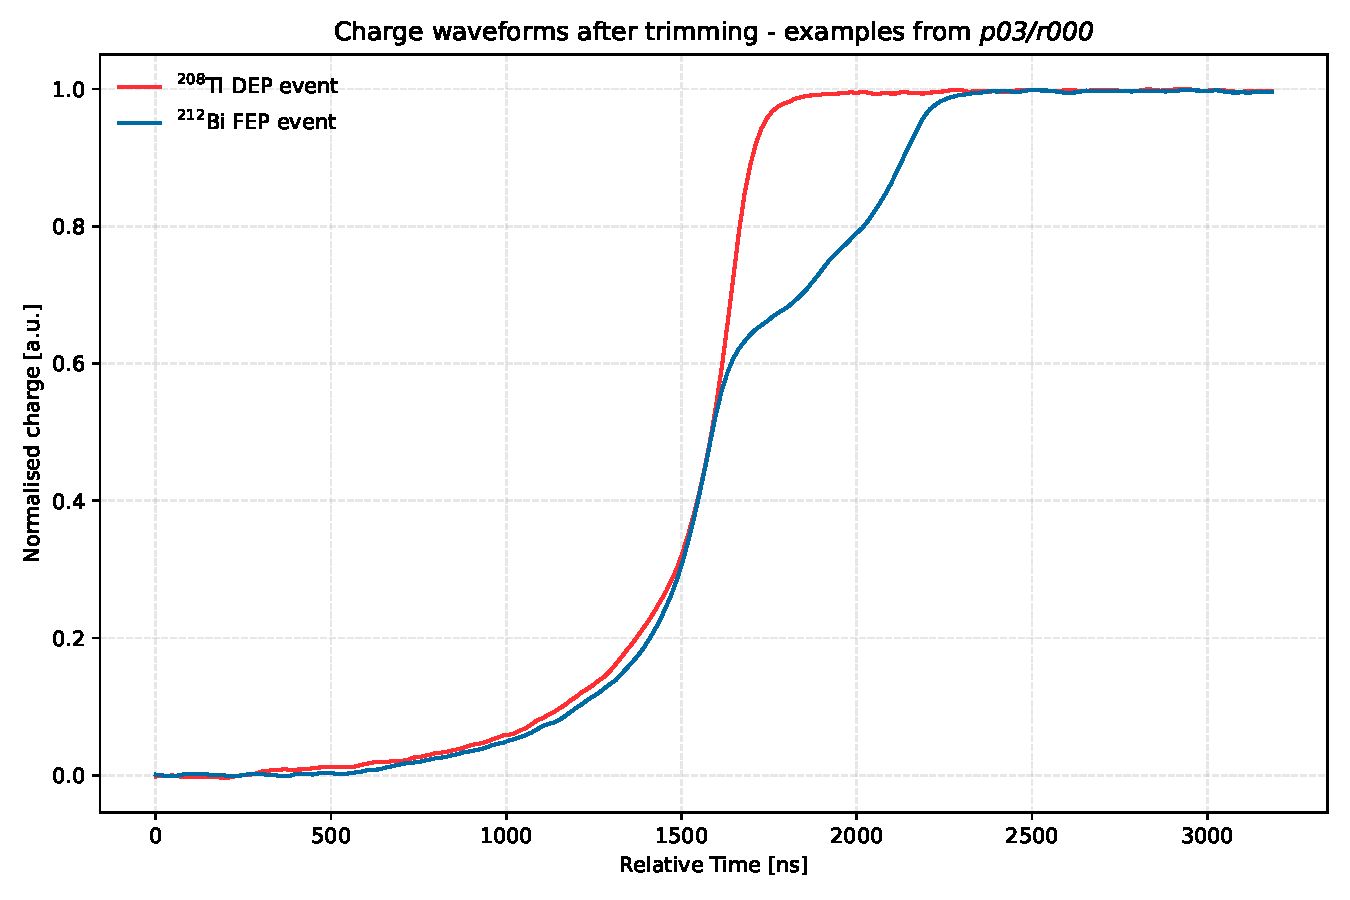
\includegraphics[width=\textwidth]{plots/trimmed_wf.pdf}
        \caption{Charge waveforms after trimming.}
        \label{fig:e-trimmed}
    \end{subfigure}
    \hfill
    % --- Sestaa figura (f) ---
    \begin{subfigure}[H]{0.45\textwidth}
        \centering
        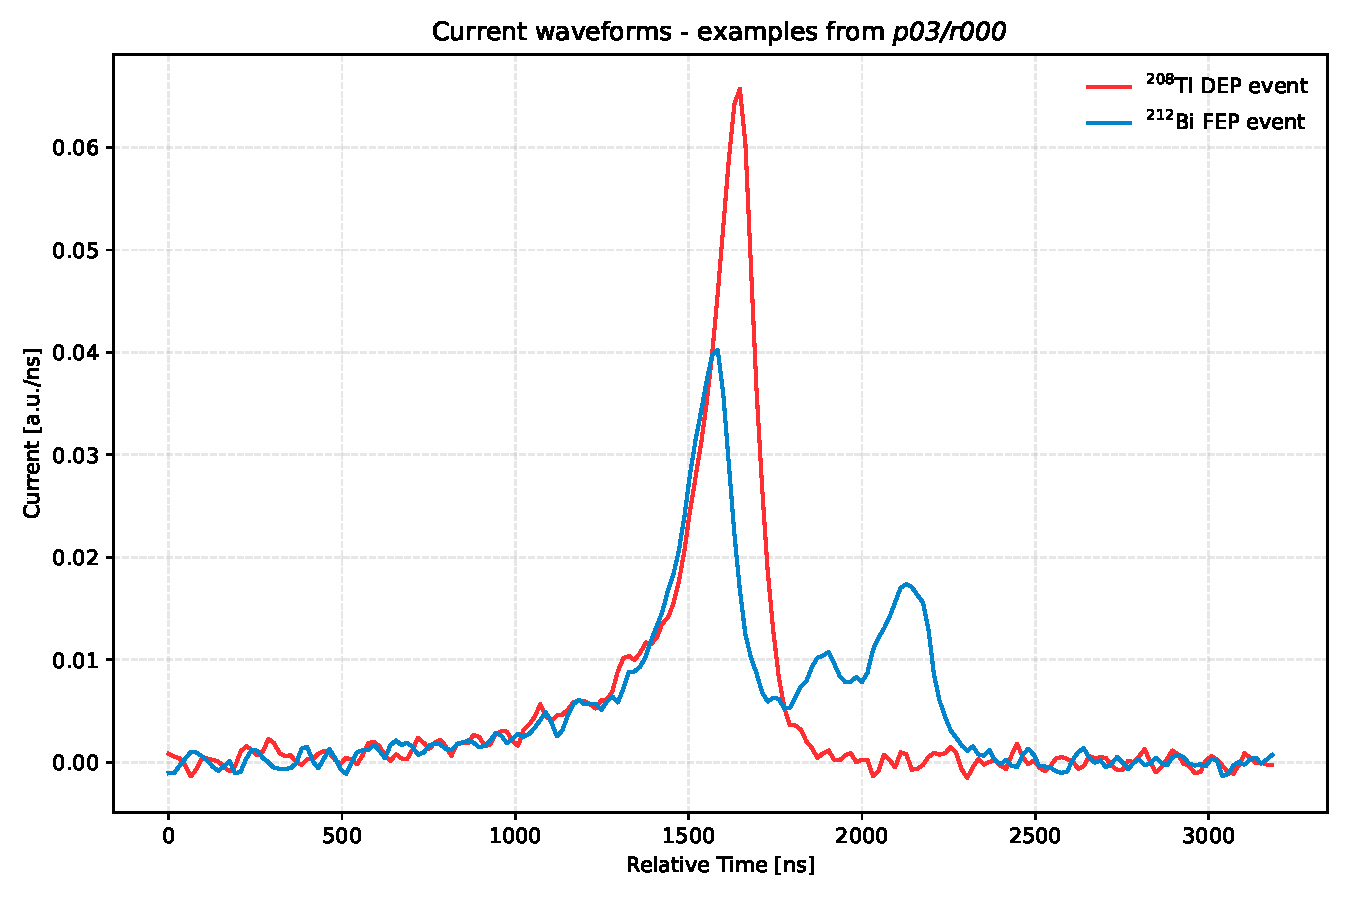
\includegraphics[width=\textwidth]{plots/current_wf.pdf}
        \caption{Current waveforms obtained with time derivative.}
        \label{fig:f-current}
    \end{subfigure}
    
    % --- Didascalia principale ---
    \caption{Illustration of the workflow of the data processing for two types of waveforms taken from run \textit{r000} of period \textit{p03}: the blue one is a typical \ac{MSE} waveform with a non-trivial structure while the orange one is a typical \ac{SSE} waveform. Raw waveforms depicted in Fig.\ref{fig:a-raw-wf} follows this procedure: the baseline, computed as the average value of the first 200 points (200 ns) is subtracted from the whole signal (\ref{fig:b-baseline}); then waveforms are then normalised to their maximum in order to have all of them between 0 and 1 (\ref{fig:c-normalised}); after they are aligned in time with the 50\% of the maximum as reference point to be aligned (\ref{fig:d-aligned}) and then trimmed in a 200 ns window around the center of the waveform, i.e. the alignement point \ref{fig:e-trimmed}. Finally the time derivative is computed in order to get the current waveforms (\ref{fig:f-current}) with which impementing the Variational Autoencoder class.}
    \label{fig:gruppo_figure}
\end{figure}

\section{Model implementation}
\label{sec:model-implementation}




\section{Results}